\subsection{Experiment 2}
\label{ssec:exp2}
\addcontentsline{toc}{section}{Experiment 2}

In this experiment we want to determine wether the number of reconfigurations
needed to succesfully complete the pushing of the box. The number of bots is
kept at 10, we see from the graphs in section~\ref{ssec:exp1} that this is a
representative number of bots. We then measure the number of reconfigurations,
which is the number of times a bot activates and performs an action.

In figure~\ref{fig:exp2-plot} we see that the number of reconfigurations is
constant under different gap sizes. It doesn't take the bots a significant
number of extra reconfigurations to cross gap.

\begin{figure}
\centering
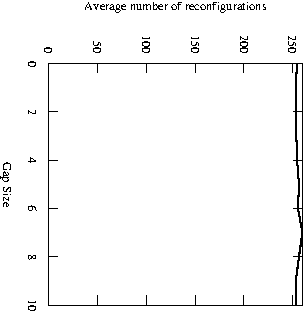
\includegraphics[width=0.6\linewidth,angle=90]{results/experiment2/plot}
\caption{The number of reconfigurations to the gap size}
\label{fig:exp2-plot}
\end{figure}

\begin{table}
 \caption{The variables involved in experiment 2.}
 \begin{center}
  \begin{tabular}{| p{5cm} | c | c |}
   \hline
   \centering \textbf{Variable} & \textbf{Type} & \textbf{Interval} \\ \hline
   gap size & independent & 0--10\\ \hline
   box weight & independent & 1 \\ \hline
   number of bots & independent & 10 \\ \hline
   number of reconfigurations &  \\ \hline
   runs per parameter set & other & 100 \\ \hline
  \end{tabular}
 \end{center}
 \label{tbl:exp2}
\end{table}
